\documentclass[12pt]{article}

\usepackage{amsmath}
\usepackage{graphicx}
\usepackage{hyperref}
\usepackage{cite}
\usepackage[margin=1.2in]{geometry}

\providecommand{\eqn}[1]{eqn.~(\ref{eqn:#1})}
\providecommand{\tab}[1]{Table~\ref{tab:#1}}
\providecommand{\fig}[1]{Figure~\ref{fig:#1}}

\title{Observing Conditions\\
during DESI Commissioning\\
\vspace{5mm}{\large\bf DESI-doc-4975-v1}}
\author{Bela Abolfathi and David Kirkby}

\begin{document}
\maketitle

\noindent {\bf Version History:}
\begin{itemize}
    \item v1: Dome open fraction from the CI run (Apr-May 2019).
\end{itemize}

\section{Introduction}

This note documents the observing conditions during the DESI Commissioning Run at the Mayall, and compares them
with the forecast model used for the survey margin estimates in DESI-4355~\cite{desi-4355}.
The periods of continuous observing during commissioning that we consider are:
\begin{itemize}
\item April 1 -- May 5, 2019: Commissioning Instrument.
\item May 16 -- June 2, 2019: Commissioning Instrument.
\end{itemize}

The latex source for this note is maintained in {\tt /doc/tex/desi4975/} of the {\tt desimodel} package on github,
with an accompanying juypter notebook in {\tt /doc/nb/CommWeather.ipynb}. This version of the document corresponds to
version {\tt 0.9.10} of the {\tt desimodel} package.

Below we describe the methods and results used to estimate the following observing conditions: dome-closed fraction,
delivered image quality, and sky transparency.  Details on the forecast models used for these quantities are in
DESI-3087~\cite{desi-3087}.

\section{Dome-Closed Fraction}

{\it Describe how the dome-closed fractions were estimated here...}

The predicted dome-closed fraction is based on the historical record for 2007--17 given in DESI-3577~\cite{desi-3577}.
We calculated the average dome-closed fraction for the nights of the CI run, April 1 -- May 5 and May 16 -- June 2, 2019.
The average of the 2007--17 predictions is 16.4\%, compared with the actual CI dome-closed fraction of 17.4\%%.
The actual weather is very consistent with the model predictions. Details are in \fig{CIdome}.

\begin{figure}[htb]
\begin{center}
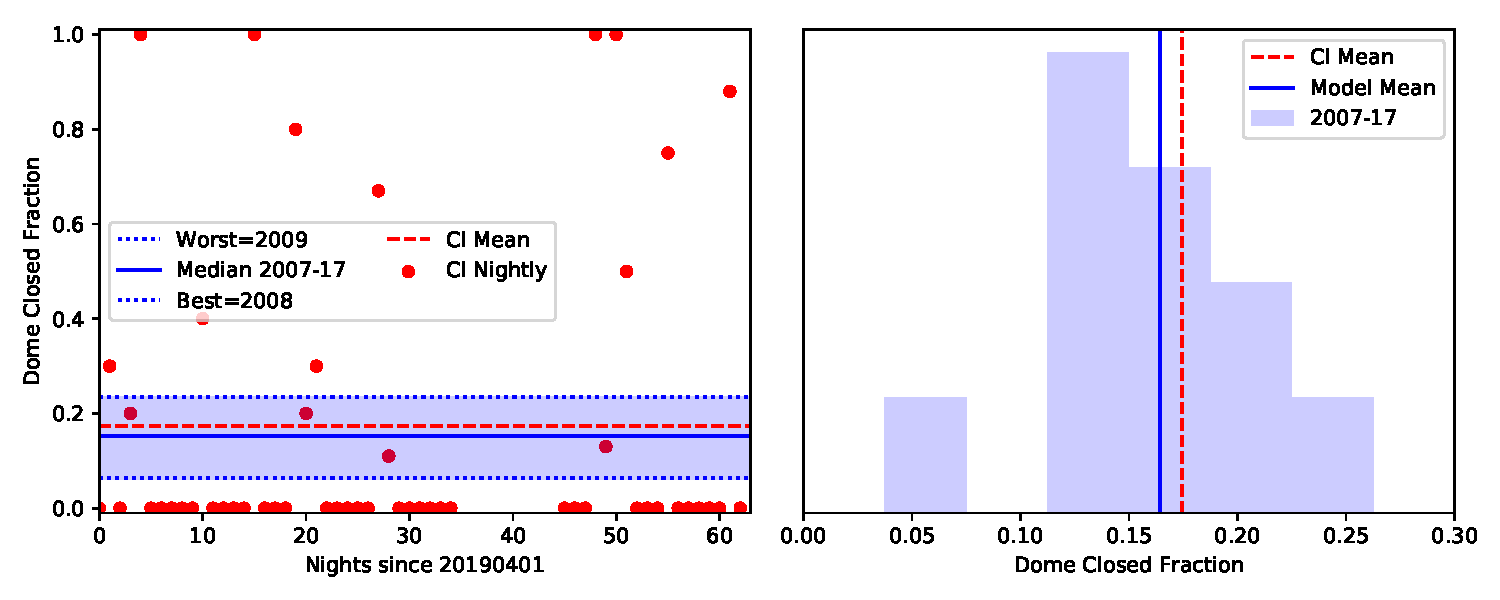
\includegraphics[width=6in]{CIdome}
\caption{Actual (red) and predicted (blue) dome-closed fraction for the dates corresponding to the CI run.}
\label{fig:CIdome}
\end{center}
\end{figure}

\section{Delivered Image Quality}

To be completed in a future version of this document.

\section{Sky Transparency}

To be completed in a future version of this document.

\bibliographystyle{unsrt}
\bibliography{CommWeather}

\end{document}
